\documentclass[oneside]{book}
\pagestyle{plain}

\usepackage{geometry}
\geometry{a4paper, portrait, margin=1.5in, top=1in, bottom=1in}

\usepackage{fontspec}
% https://fonts.google.com/specimen/IBM+Plex+Serif
\setmainfont{IBM Plex Serif}
\setmonofont{Ubuntu Mono}

\usepackage[russian]{babel}

\usepackage[fontsize=9pt]{fontsize}
\usepackage[skip=5pt plus1pt, indent=20pt]{parskip} % setup paragraphs

\usepackage{setspace}
%% \singlespacing
\onehalfspacing
%% \doublespacing

%% https://latex-tutorial.com/color-latex/
\usepackage[x11names]{xcolor}

\usepackage{graphicx}

%% https://texdoc.org/serve/listings.pdf/0
\usepackage{listings}
%% https://texdoc.org/serve/listings.pdf/0
%% 3.1 Style definitions
%% 3.2 Language definitions

\lstdefinelanguage{Elixir}{
    morekeywords={case,catch,def,do,else,false,%
        use,alias,receive,timeout,defmacro,defp,%
        for,if,import,defmodule,defprotocol,%
        nil,defmacrop,defoverridable,defimpl,%
        super,fn,raise,true,try,end,with, unless},
    morekeywords={[2]@spec, @type, assert, test},
    %% otherkeywords={<-,->, |>, \%\{, \}, \{, \, (, )},
    sensitive=true,
    morecomment=[l]{\#},
    morestring=[b]',
    morestring=[b]"
}

\lstdefinestyle{elixir}{
  %% frame=trbl,
  frame=l,
  basicstyle=\ttfamily\small,
  commentstyle=\ttfamily,
  breaklines,
  showtabs=false,
  showspaces=false,
  showstringspaces=false,
  numbers=left,
  numberstyle=\tiny,
  keywordstyle=\color{SteelBlue4}\bfseries,
  keywordstyle=[2]\color{SteelBlue4},
  identifierstyle=\color{DeepSkyBlue3},
  stringstyle=\color{SeaGreen4},
  commentstyle=\color{gray},
  backgroundcolor=\color{Ivory1}
}

\lstdefinelanguage{ElixirShell}{
    otherkeywords={iex>},
    sensitive=true,
    morecomment=[l]{\#},
    morestring=[b]',
    morestring=[b]"
}

\lstdefinestyle{elixir-shell}{
  numbers=none,
  frame=l,
  basicstyle=\ttfamily\small,
  commentstyle=\ttfamily,
  breaklines,
  showtabs=false,
  showspaces=false,
  showstringspaces=false,
  keywordstyle=\color{SteelBlue4}\bfseries,
  identifierstyle=\color{black},
  stringstyle=\color{SeaGreen4},
  backgroundcolor=\color{Cornsilk1}
}


%% it has to be the last package to be imported
\usepackage{hyperref}

\hypersetup{
    colorlinks=true,
    linkcolor=blue,
    urlcolor=blue
    }

\urlstyle{same}


\title{Язык программирования Эликсир}
\author{Юрий Жлоба}
\date{Ноябрь 2022}

%% rights: Creative Commons Attribution-NonCommercial-ShareAlike 4.0 International Public License

\begin{document}

\maketitle

%% \frontmatter
%% \chapter{Dedication}
%% \chapter{Copyright}
%% \chapter{Acknowledgements}

%% \mainmatter

\tableofcontents

\chapter{Решаем задачу FizzBuzz}

Начнем знакомство с Эликсир на примере решения задачи \name{FizzBuzz}:

\textit{Напишите программу, которая выводит на экран числа от 1 до 100. При этом вместо чисел, кратных трем, программа должна выводить слово «Fizz», а вместо чисел, кратных пяти — слово «Buzz». Если число кратно и 3, и 5, то программа должна выводить слово «FizzBuzz».}

Это простая задача позволит познакомиться со многими важными элементами языка:
\blist
\e модули и функции;
\e генерация списка с помощью \codename{Range};
\e итерация по списку с помощью \codename{Enum.each};
\e условые переходы с помощью \code{cond do};
\e охранные выражения (\code{guards});
\e вывод на консоль;
\e оператор \code{pipe};
\e и модульные тесты (\codename{Unit Tests}).
\elist

\section{Шаг 1. Простая реализация задачи.}

Создаем модуль \codename{FizzBuzz} и в нем две функции \code{main} и \code{fizzbuzz}.

\lstinputlisting[caption=FizzBuzz, language=Elixir, style=elixir]{../lesson_01/lib/fizz_buzz_01.exs}

В функции \code{main} мы генерируем последовательность от 1 до 100. Конструкция \code{1..100} -- это генератор последовательности, он называется \codename{Range}. Затем с помощью \code{Enum.each} мы применяем функцию \code{fizzbuzz} к каждому элементу.

\code{fizzbuzz} использует конструкцию \code{cond do} и охранные выражения (guards) чтобы проверить условия делимости на 3 и на 5. Первое охранное выражение выполняется, если \code{n} делится на 3 и на 5. Второе охранное выражение выполняется, если \code{n} делится на 3. Третье, если \code{n} делится на 5. И последнее, четвертое охранное выражение выполняется всегда, так как оно представлено просто значением \code{true}.

Функция \code{rem}, как не трудно догадаться, возвращает остаток от деления.

\code{cond do} проверяет выражения по очереди, и выполняет только одну ветку кода, соответствующую первому истинному выражению. \code{IO.puts} выводит нужное значение на стандартный вывод.

Соберем и запустим наш код:
\lstinputlisting[caption=Сессия 1, language=ElixirShell, style=elixir-shell]{../lesson_01/lib/session_01.txt}

\section{Шаг 2. Отделяем вывод на консоль от логики.}

Функция \code{fizzbuzz} выводит сообщения на консоль, что не очень хорошо с точки зрения функционального программирования. Разделим нашу задачу на две:

1. Преобразовать список чисел \code{1..100} в другой список, состоящий из чисел и строк: \code{Fizz, Buzz, FizzBuzz}.

2. Вывести результат на консоль.

\lstinputlisting[caption=FizzBuzz02, language=Elixir, style=elixir]{../lesson_01/lib/fizz_buzz_02.exs}

Функция \code{fizzbuzz} теперь стала \name{чистой функцией}. Её результат зависит только от входного значения, и она не делает ничего, кроме вычисления результата. Чистые функции легко понять и протестировать. А так же их легко компоновать друг с другом.

Еще мы сделали небольшую оптимизацию -- вынесли вычисление остатка от деления в отдельное выражение и сохранили результат в переменную. Таким образом мы вычисляем делимость на 3 и на 5 только один раз. В предыдущем решении мы вычисляли это несколько раз.

Мы также добавили \code{@spec} -- спецификацию функции, где описаны типы входящего значения и результата. Хотя Эликсир является языком с динамической типизацией, в нем можно указывать типы для переменных и функций. Компилятор Эликсир не проверяет типы, но есть отдельный инструмент -- \name{dialyzer}, который выполняет статический анализ кода, и в том числе проверку типов.

Вторая задача, вывод результата на консоль, реализована в функции \code{main}. Давайте посмотрим, что здесь изменилось.

Во-первых, мы заменили \code{Enum.each} на \code{Enum.map}. Оба варианта применяют функцию к каждому элементу списка. Но \code{each} игнорирует результаты, а \code{map} собирает их в новый список.

Дальше мы видим оператор \code{pipe}, который позволяет собрать несколько вызовов функций в цепочку, где результат вызова предыдущей функции передается как первый аргумент в следущую функцию. Оператор pipe и такие цепочки функций популярны в Эликсир и являются хорошей практикой.

В нашей цепочке список \code{1..100} передается в \code{Enum.map}, затем новый список передается в \code{Enum.join}, где он склеивается в одну строку. И, наконец, эта строка передается в \code{IO.puts} и выводится на консоль.

Результат выполнения кода немного изменился:

\lstinputlisting[caption=Сессия 2, language=ElixirShell, style=elixir-shell]{../lesson_01/lib/session_02.txt}

Теперь все значения склеены в одну строку, а не выводятся каждое отдельной строкой.

\section{Шаг 3. Юнит-тесты.}

Написать юнит-тест на то, что функция делает правильный вывод на консоль не тривиально. А написать юнит-тест на то, что функция возвращает правильную строку, это тривиально. Чистые функции легко тестировать.

На втором шаге у нас появилась чистая функция \code{fizzbuzz}, которая принимает одно число, и возвращает строку. Но вся задача в целом, fizzbuzz для 100 чисел, пока не представлена чистой функцией. Давайте это исправим:

\lstinputlisting[firstline=2, lastline=12, firstnumber=2, caption=FizzBuzz03, language=Elixir, style=elixir]{../lesson_01/lib/fizz_buzz_03.exs}

Функция \code{fizzbuzz\_100} не принимает аргументов и возвращает список строк. Дальше этот список мы, как и прежде, склеиваем в одну строку и выводим на консоль.

Теперь мы можем протестировать всю задачу целиком.

В Эликсир есть библиотека \name{ExUnit}, которая несмотря на свое название, позволяет писать и юнит-тесты и интеграционные тесты.

Сделаем отдельные тесты для \code{fizzbuzz} и для \code{fizzbuzz\_100}:

\lstinputlisting[firstline=28, lastline=58, firstnumber=28, caption=FizzBuzzTest, language=Elixir, style=elixir]{../lesson_01/lib/fizz_buzz_03.exs}

Как видим, \code{fizzbuzz} тестируется легко. А вот \code{fizzbuzz\_100} возвращает слишком большой список. Проверять его весь нерационально. Поэтому тест проверяет отдельные части этого списка.

\code{Enum.take} берет несколько элементов от головы списка, \code{Enum.drop} отбрасывает несколько элементов и возвращает остаток списка. Комбинация этих двух функций позволяет выделить произвольную часть списка.

Запускаем тесты:

\lstinputlisting[caption=Сессия 3, language=ElixirShell, style=elixir-shell]{../lesson_01/lib/session_03.txt}

\chapter{Интерактивная консоль}

Посмотрим на интерактивную консоль \name{iex} -- второй по важности, после редактора, инструмент разработчика.

Многие языки программирования имеют \name{REPL} консоль. Она дает возможность работать интеративно: запускать небольшие куски кода и сразу же видеть результ. REPL означает Read, Eval, Print, Loop. То есть, консоль читает код, выполняет его, выводит результат, и опять читает код.

Мы уже начали активно пользоваться консолью когда реализовывали \codename{FizzBuzz}. Теперь познакомимся с ней поближе:

\begin{lstlisting}[caption=Запуск консоли, language=ElixirShell, style=elixir-shell]
$ iex
Erlang/OTP 24 [erts-12.2.1] [source] [64-bit] [smp:12:12] [ds:12:12:10] [async-threads:1] [jit]

Interactive Elixir (1.13.3) - press Ctrl+C to exit (type h() ENTER for help)
iex>
\end{lstlisting}

Мы видим версию Эрланг: \code{Erlang/OTP 24}, версию Erlang Runtime System: \code{erts-12.2.1} и версию Эликсир: \code{Elixir (1.13.3)}.

\section{Компиляция}

iex-консоль имеет много встроенных функций. Самые популярные из них имеют однобуквенные называния.

Например, функция \name{c} компилирует и загружает код:

\begin{lstlisting}[language=ElixirShell, style=elixir-shell]
iex> c "lib/fizz_buzz_02.exs"
[FizzBuzz02]
B>
\end{lstlisting}

Другая популярная функция -- это \name{h}, которая показывает справку по функциям и модулям Эликсир. Посмотрим справку по функции \name{c}:

\begin{lstlisting}[language=ElixirShell, style=elixir-shell]
iex> h c
def c(files, path \\ :in_memory)

Compiles the given files.
...
\end{lstlisting}

Мы видим, что функция \name{c} компилирует один или несколько файлов, загружает их в память консоли, или сохраняет сгенерированный байт-код по указаному пути.

Если мы вносим изменения в код, то с помощью функции \name{r} мы можем перекомпилировать модуль заново и загрузить свежую версию.

\begin{lstlisting}[language=ElixirShell, style=elixir-shell]
iex> r FizzBuzz02
warning: redefining module FizzBuzz02 (current version defined in memory)
  lib/fizz_buzz_02.exs:1

{:reloaded, [FizzBuzz02]}
\end{lstlisting}

Таким образом удобно вести интерактивную разработку -- писать код и тут же проверять в консоли, как он работает.

Для больших проектов неудобно перекомпилировать по-отдельности каждый измененный модуль. Поэтому в консоли есть функция \name{recompile}, которая пересобирает весь проект. Однако, для этого нужно иметь полноценный проект с правильной структурой кода, а не просто несколько модулей.

\section{Автодополнение}

Для кода, который скомпилирован и загружен в консоль, работает автодополнение модулей и функций:

\begin{lstlisting}[language=ElixirShell, style=elixir-shell]
iex> Fizz.<tab>
iex> FizzBuzz02.<tab>
iex> FizzBuzz02.m<tab>
iex> FizzBuzz02.main
\end{lstlisting}

\section{Интроспекция}

Еще одна полезная функция, \name{i} -- это интроспеция, которая показывает информацию о значениях и переменных:

\begin{lstlisting}[language=ElixirShell, style=elixir-shell]
iex> i 42
Term
  42
Data type
  Integer
...

iex> i 3.14
Term
  3.14
Data type
  Float
...

iex> my_str = "Hello"
iex> i my_str
Term
  "Hello"
Data type
  BitString
Byte size
  5
Description
  This is a string: a UTF-8 encoded binary ...

iex> my_list = [1, 2, 3]
iex> i my_list
Term
  [1, 2, 3]
Data type
  List
...
\end{lstlisting}

\section{История}

Как и большинство других консолей, iex-консоль сохраняет историю команд и позволяет перемещатсья по ней с помощью горячих клавиш \code{Ctrl-p} и \code{Ctrl-n} или стрелками.

Также консоль позволяет обратиться к результатам предыдущих команд с помощью функции \name{v}. Она принимает номер строки и возвращает результат команды из этой строки. Её также можно вызвать без аргументов, тогда она вернет результат предыдущей команды:

\begin{lstlisting}[language=ElixirShell, style=elixir-shell]
iex> 42 * 2
84
iex> v
84
iex> v 9
84
iex> 20 + 30
50
iex> v
50
iex> v 12
50
iex> v 9
84
\end{lstlisting}

\section{Справка}

Рассмотрим подробнее функцию \name{h}. Если вызывать ее без аргументов, то мы увидим справку по самой консоли iex.

Аргументом можно передать имя модуля, функции или макроса. Тогда консоль покажет справку по ним:
\begin{lstlisting}[language=ElixirShell, style=elixir-shell]
iex> h
iex> h Map
iex> h Map.get
iex> h Map.<tab>
iex> h Map.fetch
\end{lstlisting}

В каждый модуль при компиляции автоматически добавляется функция \code{module\_info}, которая возращает некоторые метаданные об этом модуле. Это справедливо как для библиотечных модулей, так и для модулей, которые мы создаем сами:

\begin{lstlisting}[language=ElixirShell, style=elixir-shell]
iex> Map.module_info
[
  module: Map,
  exports: [
    __info__: 1,
    delete: 2,
    equal?: 2,
    fetch: 2,
    fetch!: 2,
...

iex> FizzBuzz02.module_info
[
  module: FizzBuzz02,
  exports: [__info__: 1, fizzbuzz: 1, main: 0, module_info: 0, module_info: 1],
  attributes: [vsn: [19328415140430776990959847375304151410]],
  compile: [
...
\end{lstlisting}


\section{Справка по собственным модулям}

Мы можем добавить документацию в собственные модули, и эта документация будет доступна в iex-консоли.

Документация для модуля задаётся с помощью аттрибута \code{@moduledoc}, а для функции с помощью аттрибута \code{@doc}:

\begin{lstlisting}[language=Elixir, style=elixir]
defmodule FizzBuzz04 do

  @moduledoc """
  FizzBuzz is a simple task to show basic usage of Elixir.
  """
  ...

  @doc "Produces list of strings for numbers from 1 to 100."
  @spec fizzbuzz_100() :: [String.t]
  def fizzbuzz_100() do
    1..100
    |> Enum.map(&fizzbuzz/1)
  end
  ...
\end{lstlisting}
Однако это не работает, если модуль просто скомпилирован из консоли:

\begin{lstlisting}[language=ElixirShell, style=elixir-shell]
iex> c "lib/fizz_buzz_04.exs"
iex> h FizzBuzz04
FizzBuzz04 was not compiled with docs
\end{lstlisting}

Нужно, чтобы скомпилированный байткод был сохранён на диске. Для этого функцию \name{c} вызываем с двумя аргументами, кроме файла исходников ещё указываем путь, куда сохранять beam-файл:

\begin{lstlisting}[language=ElixirShell, style=elixir-shell]
iex> c("lib/fizz_buzz_04.exs", ".")
iex> h FizzBuzz04
FizzBuzz04

FizzBuzz is a simple task to show basic usage of Elixir.

iex> h FizzBuzz04.fizzbuzz_100

def fizzbuzz_100()

@spec fizzbuzz_100() :: [String.t()]

Produces list of strings for numbers from 1 to 100.

iex> h FizzBuzz04.fizzbuzz

 def fizzbuzz(n)

@spec fizzbuzz(integer()) :: String.t()

Produces string result for a single number.
\end{lstlisting}

\section{runtime\_info}

Рассмотрим еще функцию \code{runtime\_info}. Длинное название этой функции подразумевает, что она не используется так же часто, как \name{c}, \name{h}, \name{i} или \name{v}.

Функция выводит полезную информацию о текущем состоянии виртуальной машины: версии Эликсир и Эрлаг, количество планировщиков, потребление памяти, количество процессов и др.

\begin{lstlisting}[language=ElixirShell, style=elixir-shell]
iex> runtime_info
## System and architecture

Elixir version:     1.13.4
Erlang/OTP version: 23
...

## Memory

Total:              20 MB
Atoms:              328 KB
...

## Statistics / limits

Uptime:             1 minutes and 40 seconds
...

iex> runtime_info :system

## System and architecture

Elixir version:     1.13.4
Erlang/OTP version: 23
ERTS version:       11.1
Compiled for:       x86_64-unknown-linux-gnu
Schedulers:         8
Schedulers online:  8
...

iex> runtime_info :memory

## Memory

Total:              20 MB
Atoms:              328 KB
Binaries:           111 KB
Code:               7 MB
ETS:                510 KB
Processes:          4 MB
...
\end{lstlisting}

Как видно, iex-консоль очень полезна. Опытные разработчики активно ей пользуются.

\chapter{Немного истории}

Эликсир молодой язык, он создан в 2012 году. Но начать я хочу за 100 лет до этого. 

\section{Предыстория: начало ХХ века.}

В начале ХХ века в Дании, в Копенгагенской телефонной компании работал инженер \href{https://ru.wikipedia.org/wiki/%D0%AD%D1%80%D0%BB%D0%B0%D0%BD%D0%B3,_%D0%90%D0%B3%D0%BD%D0%B5%D1%80_%D0%9A%D1%80%D0%B0%D1%80%D1%83%D0%BF}{Агнер Краруп Эрланг}

\begin{figure}[h]
  \centering
  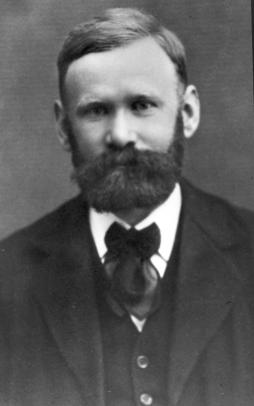
\includegraphics[width=0.3\textwidth]{../lesson_02/img/agner_krarup_erlang.jpg}
  \caption{Agner Krarup Erlang}
\end{figure}

Его интересовало, как наиболее эффективным образом использовать оборудование телефонной станции, чтобы обслуживать максимальное количество абонентов.

Агнер Эрланг был хорошо образован, с отличием закончил университет, и умел применять в работе методы математики и статистики. И он не ленился самостоятельно залезать на телефонные столбы, чтобы собрать нужные данные.

Результатом его усилий стала научная работа \href{https://ru.wikipedia.org/wiki/%D0%A2%D0%B5%D0%BE%D1%80%D0%B8%D1%8F_%D0%BC%D0%B0%D1%81%D1%81%D0%BE%D0%B2%D0%BE%D0%B3%D0%BE_%D0%BE%D0%B1%D1%81%D0%BB%D1%83%D0%B6%D0%B8%D0%B2%D0%B0%D0%BD%D0%B8%D1%8F}{"Теория массового обслуживания"}. Она позволяет рационально расчитать ресурсы, необходимые для обслуживания требований, поступающих в систему, исходя из длительности ожидания и длины очередей.

Теория применяется не только в телекоммуникационных системах, а гораздо шире: в управлении автомобильным и воздушным движением, на конвейерном производстве, в логистике, а также при проектировании фабрик, складов, магазинов и больниц.

В честь Агнера Эрланга названы единица измерения трафика в телекоммуникационных системах и язык программирования.

\section{История Эрланг: c 1985 по настоящее время.}

\begin{figure}[h]
  \centering
  
\includegraphics[width=0.3\textwidth]{../lesson_02/img/erlang_logo.png}
  \caption{Erlang}
\end{figure}

Язык \textbf{Эрланг} родился в недрах шведской компании Эрикссон (Ericsson) -- крупного поставщика телекомуникационного оборудования и услуг.

Для этой индустрии характерны сложное оборудование, сложный софт, большой траффик и жесткие требования по доступности сервиса.

В компании был отдел, занимающийся научной работой: \textit{Ericsson’s Computer Science Laboratory}. Отделу была поставлена задача найти более эффективные средства разработки софта для железа и сервисов компании.

У компании уже был опыт разработки языков программирования. Использовались собственные проприетарные языки \textit{PLEX} и \textit{EriPascal}. Но они не стремились разработать еще один язык, а хотели найти подходящее решение среди уже существующих.

В течение 2х лет отдел писал прототипы телеком-приложений на разных языках, имеющихся в то время:
\begin{itemize}
\item функциональные языки \textit{ML} и \textit{Miranda};
\item многопоточные языки \textit{ADA}, \textit{Modula} и \textit{Chill};
\item логический язык \textit{Prolog};
\item объектно-ориентированный \textit{Smalltalk}.
\end{itemize}

Разработчики пришли к выводу, что ни один язык не имеет нужных возможностей. И главная проблема была в реализации многопоточности на нужном уровне. В итоге лаборатория решила разработать свой язык программирования.

В отличие от большинства языков, разработанных для "общего" применения и на "правильном" теоретическом базисе, Эрланг изначально разрабатывался для узкого применения, исходя из практических требований. От этого идут его преимущества и недостатки.

В 1998 Эрланг был выпущен в open source, и стал известен за пределами Эрикссон. Следующие несколько лет он использовался в Эрикссон, и отдельными энтузиастами за пределами компании, но был мало известен.

В 2002 году был начат проект \textbf{ejabberd} -- первый крупный open source проект на Эрланг. Он стал основой для большинства IM (Instant Messaging) систем, в т.ч. для широко известного \textbf{WhatsApp}.

В 2006 году в появилась поддержка симметричной мультипроцессорности (SMP). Эрланг научился эффективно использовать все имеющиеся в системе процессорные ядра.

И это случилось в подходящий момент. К этому времени производители процессоров достигли предела тактовых частот. Дальше наращивать мощность одного процессора было невозможно, и производители пошли по пути увеличения числа процессоров.

А у IT-индустрии появилась потребность разрабатывать многопоточные программы, эффективно использующие несколько процессоров. Делать это на популярных языках программирования было трудно, и возник интерес к функциональному программированию вообще, и к Эрланг в частности.

Этот интерес проявился в двух направлениях:
\begin{itemize}
\item стали шире использоваться ФП языки;
\item популярные языки начали заимствовать идеи ФП и реализовывать их у себя.
\end{itemize}

В 2007 вышла книга Джо Армстронга "Programming Erlang".

Нынче Эрланг известен и применяется достаточно широко.

\section{История Эликсир: c 2012 по настоящее время.}

\begin{figure}[h]
  \centering
  
\includegraphics[width=0.3\textwidth]{../lesson_02/img/elixir_logo.png}
  \caption{Elixir}
\end{figure}

\textbf{Эликсир} создан в 2012 году как исследовательский проект в компании Plataformatec. Его автор -- \textbf{Жозе Валим}, был одним из основных разработчиков фреймворка \textit{Ruby on Rails} и сооснователем компании \textit{Plataformatec}.

Авторы языка имели большой опыт веб-разработки на разных языках и с разными фреймворками. Как это обычно бывает, они постарались собрать в одном языке все лучшее из своего опыта.

Эликсир позаимствовал идеи из Ruby, Clojure и Эрланг. Большое влияние оказали Ruby и фрейморк Ruby on Rails. Система макросов заимствована из Clojure. Ну и, конечно, Эликсир унаследовал все возможности Эрланг и его виртуальной машины.

Почти одновременно с Эликсир создавались \textit{Ecto} -- библиотека для работы с реляционными базами данных и фреймворк \textit{Phoenix}.

Первая версия языка вышла в 2014 году. Немного позже, в 2015 году, вышли первые версии Ecto и Phoenix. С тех пор язык и библиотеки активно развиваются. Вокруг них сформировалось большое сообщество.

\chapter{Типы данных}

Любой язык программирования начинается с базовых типов данных и операций над ними.

Из базовых типов строятся более сложные типы, которые тоже имеют свой набор операций.

Наконец, из базовых и сложных типов можно создавать новые, пользовательские типы данных, и реализовывать новые операции над ними.

В этом уроке мы начнем знакомиться с базовыми типами.

number
  integer
  float

boolean

atom

collections
  tuple
  list
  map
  string/binary

system types
  pid
  port
  reference
  function
  
complex types
  io list
  keyword list
  range
  sigil: Date, Time, DateTime, RE
  


%% \backmatter
%% \chapter{Bibliography}
%% \chapter{Other titles in this collection}

\end{document}
